\documentclass[11pt, a4paper]{article}

% Fonts and Encoding
\usepackage[utf8]{inputenc}
\usepackage[T1]{fontenc}

% Math and Symbols
\usepackage{amsmath, amssymb, amsthm, amsfonts, mathrsfs, mathtools}

% Layout and Geometry
\usepackage{geometry}
\geometry{a4paper, margin=1in}

% Formatting and Graphics
\usepackage{graphicx, xcolor, enumitem, booktabs, array, tabularx}

% TikZ for Illustrations
\usepackage{tikz}
\usetikzlibrary{arrows.meta, positioning, shapes.geometric, calc, backgrounds, matrix}

% Clickable Links and TOC
\usepackage{hyperref}
\hypersetup{
    colorlinks=true,
    linkcolor=blue,
    filecolor=magenta,      
    urlcolor=cyan,
    pdftitle={Proof by Minimum Counterexample},
}

% Theorem Environments
\newtheorem{theorem}{Theorem}[section]
\newtheorem{lemma}[theorem]{Lemma}
\newtheorem{proposition}[theorem]{Proposition}
\newtheorem{corollary}[theorem]{Corollary}
\theoremstyle{definition}
\newtheorem{definition}{Definition}[section]
\newtheorem{axiom}{Axiom}[section]
\newtheorem{example}{Example}[section]
\theoremstyle{remark}
\newtheorem{remark}{Remark}[section]

% Custom Commands (Enforced standard notation)
\newcommand{\R}{\mathbb{R}}
\newcommand{\N}{\mathbb{N}}
\newcommand{\Z}{\mathbb{Z}}
\newcommand{\Q}{\mathbb{Q}}
\newcommand{\E}{\mathbb{E}}
\newcommand{\Prob}{\mathbb{P}}
\newcommand{\F}{\mathcal{F}}

\title{\textbf{Advanced Mathematical Induction: \\ Proof by Minimum Counterexample}}
\author{Tashfeen Omran}
\date{\today}

\begin{document}

\maketitle
\tableofcontents
\newpage

\section{Comprehensive Introduction, Context, and Prerequisites}

\subsection{Core Concepts \& Axioms}
In the foundational study of abstract mathematics, the integers possess a rigid, discrete topological structure that allows for powerful logical deductions. The method of \textbf{Proof by Minimum Counterexample} is a sophisticated variant of Mathematical Induction. It relies entirely on a fundamental axiom of the natural numbers known as the \textbf{Well-Ordering Principle (WOP)}.

\begin{axiom}[The Well-Ordering Principle]
Every non-empty subset of the natural numbers $\N$ contains a least element. Formally, if $S \subseteq \N$ and $S \neq \emptyset$, then there exists an element $m \in S$ such that $m \le x$ for all $x \in S$.
\end{axiom}

The logical architecture of a Proof by Minimum Counterexample to prove a proposition $P(n)$ for all $n \in \N$ proceeds as follows:
\begin{enumerate}
    \item \textbf{Assumption of Falsity:} Assume, for the sake of contradiction, that $P(n)$ is false for at least one $n \in \N$.
    \item \textbf{Set Construction:} Define the set of all counterexamples: $S = \{ n \in \N : P(n) \text{ is false} \}$. By our assumption, $S \neq \emptyset$.
    \item \textbf{Invocation of WOP:} By the Well-Ordering Principle, $S$ must have a minimum element, say $m$. Thus, $m$ is the \textit{smallest} integer for which $P(m)$ is false.
    \item \textbf{Minimality Exploitation:} Because $m$ is the absolute minimum of $S$, it strictly follows that for any positive integer $k < m$, $k \notin S$. Therefore, $P(k)$ must be \textit{true}.
    \item \textbf{Contradiction Generation:} Using the truth of $P(k)$ (often $P(m-1)$), logically deduce that $P(m)$ must also be true, or construct an even smaller counterexample $m' < m$ such that $P(m')$ is false. Both outcomes contradict the definition of $m$, forcing the conclusion that $S = \emptyset$.
\end{enumerate}

\subsection{Intuition and Set-Theoretic Foundations}
Intuitively, imagine a staircase descending into an abyss. If a property fails at some step, there must be a \textit{first} step where it fails. If we can prove that the failure at this "first" step logically necessitates a failure at an even earlier step, we create an impossible infinite descent within a space bounded below by $1$. In set-theoretic terms, we are demonstrating that the assumption of a non-empty complement to the truth set of $P(n)$ violates the order-isomorphism of $\N$.

\subsection{Historical Context and Motivation}
The formalization of the Well-Ordering Principle dates back to Giuseppe Peano's axioms (1889) and later Ernst Zermelo's Well-Ordering Theorem (1904), which proved that \textit{every} set can be well-ordered, assuming the Axiom of Choice. In number theory, Pierre de Fermat famously utilized a specialized version of this technique called the "Method of Infinite Descent" in the 17th century to prove cases of his Last Theorem. Fermat realized that if a solution to a Diophantine equation existed, he could algebraically construct a strictly smaller integer solution, leading to an impossible infinite sequence of decreasing positive integers.

\subsection{Prerequisites}
To master this module, the reader must possess:
\begin{itemize}
    \item \textbf{Foundational Logic:} Mastery of Proof by Contradiction ($A \implies \bot \vdash \neg A$).
    \item \textbf{Algebraic Manipulation:} Proficiency in polynomial expansion, factoring, and telescoping sums.
    \item \textbf{Modular Arithmetic \& Divisibility:} Understanding of the definition of divisibility ($a \mid b \iff \exists k \in \Z, b = ak$).
\end{itemize}

\newpage
\section{Detailed Homework Solutions}

In this section, we provide rigorous, step-by-step proofs for Exercises 6.40 through 6.47 from the provided text. Every proof utilizes the Method of Minimum Counterexample.

\subsection{Exercise 6.40}
\textbf{Problem:} Use the method of minimum counterexample to prove Result 6.23: If $r$ is a nonzero real number such that $r + \frac{1}{r}$ is an integer, then $r^n + \frac{1}{r^n}$ is an integer for every positive integer $n$.

\begin{proof}
Assume, to the contrary, that there exists a nonzero real number $r$ such that $r + \frac{1}{r} \in \Z$, but $r^n + \frac{1}{r^n} \notin \Z$ for some positive integer $n$. Let $S$ be the set of all such positive integers $n$. Since $S$ is non-empty, the Well-Ordering Principle guarantees that $S$ has a minimum element, say $m$. 

We first check the base cases. 
For $n=1$, $r^1 + \frac{1}{r^1} = r + \frac{1}{r} \in \Z$ by hypothesis. Thus, $1 \notin S$.
For $n=2$, observe that $\left(r + \frac{1}{r}\right)^2 = r^2 + 2 + \frac{1}{r^2}$. Rearranging yields $r^2 + \frac{1}{r^2} = \left(r + \frac{1}{r}\right)^2 - 2$. Since $r + \frac{1}{r} \in \Z$, its square is an integer, and subtracting $2$ yields an integer. Thus, $2 \notin S$.

Therefore, the minimum counterexample $m$ must satisfy $m \ge 3$. Because $m$ is the minimum element of $S$, the statement holds for all positive integers $k < m$. Specifically, it holds for $k = m-1$ and $k = m-2$. Hence, both $\left(r^{m-1} + \frac{1}{r^{m-1}}\right)$ and $\left(r^{m-2} + \frac{1}{r^{m-2}}\right)$ are integers.

Consider the product of the $(m-1)$-th term and the $1$-st term:
\[
\left(r^{m-1} + \frac{1}{r^{m-1}}\right)\left(r + \frac{1}{r}\right) = r^m + r^{m-2} + \frac{1}{r^{m-2}} + \frac{1}{r^m}
\]
Isolating the $m$-th term, we obtain:
\[
r^m + \frac{1}{r^m} = \left(r^{m-1} + \frac{1}{r^{m-1}}\right)\left(r + \frac{1}{r}\right) - \left(r^{m-2} + \frac{1}{r^{m-2}}\right)
\]
Since $\left(r^{m-1} + \frac{1}{r^{m-1}}\right) \in \Z$, $\left(r + \frac{1}{r}\right) \in \Z$, and $\left(r^{m-2} + \frac{1}{r^{m-2}}\right) \in \Z$, the right side of the equation is a combination of integers under multiplication and subtraction, which is closed over $\Z$. Therefore, $r^m + \frac{1}{r^m} \in \Z$. This contradicts the assumption that $m \in S$. Thus, $S$ must be empty.
\end{proof}

\subsection{Exercise 6.41}
\textbf{Problem:} Give a proof by minimum counterexample that $1 + 3 + 5 + \dots + (2n - 1) = n^2$ for every positive integer $n$.

\begin{proof}
Assume, to the contrary, that the formula does not hold for all positive integers. Let $S = \{ n \in \N : 1 + 3 + \dots + (2n - 1) \neq n^2 \}$. By the Well-Ordering Principle, $S$ has a minimum element, $m$.

For $n=1$, the left side is $2(1)-1 = 1$, and the right side is $1^2 = 1$. Since $1 = 1$, the formula holds for $n=1$. Thus, $m \ge 2$.

Since $m$ is the minimum counterexample, the formula must be true for $m-1$. Therefore:
\[
1 + 3 + 5 + \dots + (2(m-1) - 1) = (m-1)^2
\]
We now evaluate the sum for $m$ by adding the $m$-th term, which is $2m - 1$, to both sides:
\[
1 + 3 + 5 + \dots + (2m - 3) + (2m - 1) = (m-1)^2 + (2m - 1)
\]
Expanding the right side:
\[
(m-1)^2 + 2m - 1 = m^2 - 2m + 1 + 2m - 1 = m^2
\]
This shows that $1 + 3 + \dots + (2m - 1) = m^2$, which means the formula holds for $m$. This contradicts the assumption that $m \in S$. Hence, $S = \emptyset$.
\end{proof}

\subsection{Exercise 6.42}
\textbf{Problem:} Prove that $5 \mid (n^5 - n)$ for every integer $n$.

\begin{proof}
We first prove the statement for all non-negative integers $n \ge 0$ using a minimum counterexample. Assume, to the contrary, that there exists a non-negative integer $n$ such that $5 \nmid (n^5 - n)$. Let $m$ be the smallest such non-negative integer.

For $n=0$, $0^5 - 0 = 0$, and $5 \mid 0$. Thus, $m \ge 1$.
For $n=1$, $1^5 - 1 = 0$, and $5 \mid 0$. Thus, $m \ge 2$.

Since $m$ is the minimum counterexample, the statement holds for $m-1$. That is, $5 \mid ((m-1)^5 - (m-1))$. By definition, there exists an integer $k$ such that $(m-1)^5 - (m-1) = 5k$.

We expand $(m-1)^5 - (m-1)$ using the Binomial Theorem:
\[
(m-1)^5 - (m-1) = (m^5 - 5m^4 + 10m^3 - 10m^2 + 5m - 1) - m + 1
\]
Grouping the terms, we get:
\[
(m-1)^5 - (m-1) = (m^5 - m) - 5(m^4 - 2m^3 + 2m^2 - m)
\]
Rearranging to isolate $m^5 - m$:
\[
m^5 - m = ((m-1)^5 - (m-1)) + 5(m^4 - 2m^3 + 2m^2 - m)
\]
Substitute $((m-1)^5 - (m-1)) = 5k$:
\[
m^5 - m = 5k + 5(m^4 - 2m^3 + 2m^2 - m) = 5 \left( k + m^4 - 2m^3 + 2m^2 - m \right)
\]
Since $k + m^4 - 2m^3 + 2m^2 - m$ is an integer, it follows that $5 \mid (m^5 - m)$. This contradicts the assumption that $m$ is a counterexample. Thus, the statement holds for all $n \ge 0$.

For negative integers, let $n = -p$ where $p > 0$. Then $n^5 - n = (-p)^5 - (-p) = -p^5 + p = -(p^5 - p)$. Since $p \ge 0$, we know $5 \mid (p^5 - p)$, which implies $5 \mid -(p^5 - p)$. Thus, the statement holds for all integers $n$.
\end{proof}

\subsection{Exercise 6.43}
\textbf{Problem:} Use proof by minimum counterexample to prove that $3 \mid (2^n + 2^{n+1})$ for every non-negative integer $n$.

\begin{proof}
Assume, to the contrary, that there exists a non-negative integer $n$ such that $3 \nmid (2^n + 2^{n+1})$. Let $m$ be the smallest such non-negative integer.

For $n=0$, $2^0 + 2^1 = 1 + 2 = 3$. Since $3 \mid 3$, $m \neq 0$. Thus, $m \ge 1$.

Because $m$ is the minimum counterexample, the statement is true for $m-1$. Therefore, $3 \mid (2^{m-1} + 2^m)$. This means there exists an integer $k$ such that $2^{m-1} + 2^m = 3k$.

We now examine the expression for $m$:
\[
2^m + 2^{m+1} = 2 \cdot 2^{m-1} + 2 \cdot 2^m = 2(2^{m-1} + 2^m)
\]
Substituting our inductive hypothesis:
\[
2^m + 2^{m+1} = 2(3k) = 3(2k)
\]
Since $2k$ is an integer, $3 \mid (2^m + 2^{m+1})$. This contradicts the assumption that $m$ is a counterexample. Hence, no such counterexample exists.
\end{proof}

\subsection{Exercise 6.44}
\textbf{Problem:} Give a proof by minimum counterexample that $2^n > n^2$ for every integer $n \ge 5$.

\begin{proof}
Assume, to the contrary, that the inequality $2^n > n^2$ is false for some integer $n \ge 5$. Let $m$ be the smallest integer greater than or equal to $5$ for which $2^m \le m^2$.

For $n=5$, $2^5 = 32$ and $5^2 = 25$. Since $32 > 25$, the inequality holds for $n=5$. Thus, $m \ge 6$.

Because $m$ is the minimum counterexample, the inequality holds for $m-1$. Therefore:
\[
2^{m-1} > (m-1)^2
\]
Multiplying both sides by $2$ yields:
\[
2^m > 2(m-1)^2 = 2(m^2 - 2m + 1) = 2m^2 - 4m + 2
\]
We wish to show that $2m^2 - 4m + 2 \ge m^2$. This is equivalent to showing that $m^2 - 4m + 2 \ge 0$.
We can rewrite this quadratic expression as:
\[
m^2 - 4m + 2 = m(m - 4) + 2
\]
Since $m \ge 6$, we have $m > 0$ and $m - 4 \ge 2$. Therefore:
\[
m(m - 4) + 2 \ge 6(2) + 2 = 14 > 0
\]
Thus, $2m^2 - 4m + 2 > m^2$. Combining this with our earlier inequality $2^m > 2m^2 - 4m + 2$, we obtain:
\[
2^m > m^2
\]
This contradicts the assumption that $2^m \le m^2$. Therefore, no such counterexample exists.
\end{proof}

\subsection{Exercise 6.45}
\textbf{Problem:} Prove that $12 \mid (n^4 - n^2)$ for every positive integer $n$.

\begin{proof}
Assume, to the contrary, that there exists a positive integer $n$ such that $12 \nmid (n^4 - n^2)$. Let $m$ be the smallest such positive integer.

For $n=1$, $1^4 - 1^2 = 0$, and $12 \mid 0$. Thus, $m \ge 2$.

Since $m$ is the minimum counterexample, the statement holds for $m-1$. Thus, $12 \mid ((m-1)^4 - (m-1)^2)$. 
Let us analyze the difference between the expression evaluated at $m$ and at $m-1$:
\[
\Delta = (m^4 - m^2) - ((m-1)^4 - (m-1)^2)
\]
Expanding $(m-1)^4$ and $(m-1)^2$:
\[
(m-1)^4 = m^4 - 4m^3 + 6m^2 - 4m + 1
\]
\[
(m-1)^2 = m^2 - 2m + 1
\]
Subtracting the two:
\[
(m-1)^4 - (m-1)^2 = m^4 - 4m^3 + 5m^2 - 2m
\]
Now, compute the difference $\Delta$:
\[
\Delta = (m^4 - m^2) - (m^4 - 4m^3 + 5m^2 - 2m) = 4m^3 - 6m^2 + 2m
\]
We can factor $\Delta$:
\[
\Delta = 2m(2m^2 - 3m + 1) = 2m(2m-1)(m-1)
\]
We must show that $12 \mid \Delta$, which is equivalent to showing $6 \mid m(2m-1)(m-1)$.
Notice that $m(m-1)$ is the product of two consecutive integers, so it is always divisible by $2$. Thus, $2 \mid m(2m-1)(m-1)$.
Next, we check divisibility by $3$. By the division algorithm, $m$ leaves a remainder of $0, 1,$ or $2$ when divided by $3$:
\begin{itemize}
    \item If $m \equiv 0 \pmod 3$, then $3 \mid m$.
    \item If $m \equiv 1 \pmod 3$, then $3 \mid (m-1)$.
    \item If $m \equiv 2 \pmod 3$, then $2m-1 \equiv 2(2)-1 = 3 \equiv 0 \pmod 3$, so $3 \mid (2m-1)$.
\end{itemize}
In all cases, $3 \mid m(2m-1)(m-1)$. Since $\gcd(2,3)=1$, it follows that $6 \mid m(2m-1)(m-1)$, and therefore $12 \mid \Delta$.
Since $(m^4 - m^2) = ((m-1)^4 - (m-1)^2) + \Delta$, and $12$ divides both terms on the right, $12 \mid (m^4 - m^2)$. This contradicts the assumption that $m$ is a counterexample.
\end{proof}

\subsection{Exercise 6.46}
\textbf{Problem:} Let $S = \{2^n : n \in \Z, n \ge 0\}$. Use proof by minimum counterexample to prove that for every $n \in \N$, there exists a subset $S_n$ of $S$ such that $\sum_{i \in S_n} i = n$.

\begin{proof}
Assume, to the contrary, that there exists a positive integer $n$ that cannot be expressed as the sum of distinct elements of $S$ (i.e., distinct powers of $2$). Let $m$ be the smallest such positive integer.

For $n=1$, $1 = 2^0 \in S$. We can choose $S_1 = \{2^0\}$, and the sum is $1$. Thus, $m \ge 2$.

Since $m \ge 2$, there exists a unique integer $k \ge 1$ such that $2^k \le m < 2^{k+1}$. 
Let $m' = m - 2^k$. Because $2^k \le m < 2^{k+1}$, we have:
\[
0 \le m' = m - 2^k < 2^{k+1} - 2^k = 2^k
\]
If $m' = 0$, then $m = 2^k$, which means $m \in S$, and we can simply choose $S_m = \{2^k\}$, a contradiction.
If $m' > 0$, then since $m' < m$, the minimality of $m$ guarantees that $m'$ \textit{can} be written as the sum of distinct elements of $S$. Let $S_{m'} \subset S$ be this subset such that $\sum_{i \in S_{m'}} i = m'$.

Because $m' < 2^k$, the largest power of $2$ that can possibly be in $S_{m'}$ is strictly less than $2^k$. Therefore, $2^k \notin S_{m'}$.
We can now construct $S_m = S_{m'} \cup \{2^k\}$. Since $2^k \notin S_{m'}$, all elements in $S_m$ are distinct. The sum of the elements in $S_m$ is:
\[
\sum_{i \in S_m} i = \left( \sum_{i \in S_{m'}} i \right) + 2^k = m' + 2^k = m
\]
This proves that $m$ can be written as the sum of distinct elements of $S$, contradicting the assumption that $m$ is a counterexample. Thus, every positive integer can be represented as a sum of distinct powers of $2$ (this is the foundation of the binary numeral system).
\end{proof}

\subsection{Exercise 6.47}
\textbf{Problem:} Use proof by minimum counterexample to prove that $6 \mid 7n(n^2 - 1)$ for every positive integer $n$.

\begin{proof}
Assume, to the contrary, that there exists a positive integer $n$ such that $6 \nmid 7n(n^2 - 1)$. Let $m$ be the smallest such positive integer.

For $n=1$, $7(1)(1^2 - 1) = 0$. Since $6 \mid 0$, $m \ge 2$.

Because $m$ is the minimum counterexample, the statement holds for $m-1$. Thus, $6 \mid 7(m-1)((m-1)^2 - 1)$.
Let us expand the expression for $m-1$:
\[
7(m-1)((m-1)^2 - 1) = 7(m-1)(m^2 - 2m) = 7(m^3 - 3m^2 + 2m) = 7m^3 - 21m^2 + 14m
\]
We want to analyze the expression for $m$, which is $7m(m^2 - 1) = 7m^3 - 7m$.
Consider the difference $\Delta$ between the expression for $m$ and the expression for $m-1$:
\[
\Delta = (7m^3 - 7m) - (7m^3 - 21m^2 + 14m) = 21m^2 - 21m = 21m(m-1)
\]
We must determine if $6 \mid \Delta$. Notice that $m(m-1)$ is the product of two consecutive integers, so it is always even. Let $m(m-1) = 2k$ for some integer $k$.
Then $\Delta = 21(2k) = 42k = 6(7k)$.
Since $7k$ is an integer, $6 \mid \Delta$.

We can express the term for $m$ as:
\[
7m(m^2 - 1) = 7(m-1)((m-1)^2 - 1) + \Delta
\]
Since $6$ divides both terms on the right side, it must divide their sum. Therefore, $6 \mid 7m(m^2 - 1)$, which contradicts the assumption that $m$ is a counterexample.
\end{proof}

\newpage
\section{In-Depth Analysis of Problems and Techniques}

\subsection{A) Problem Types and Logical Strategies}
The problems solved in the previous section fall into three distinct mathematical categories, each requiring a tailored strategic approach when applying the Minimum Counterexample method:

\begin{enumerate}
    \item \textbf{Divisibility Proofs (Ex 6.42, 6.43, 6.45, 6.47):} 
    \textit{Strategy:} The overarching goal is to express the function evaluated at the counterexample $m$, denoted $f(m)$, in terms of $f(m-1)$ plus a residual term $\Delta$. Because $m$ is the minimum counterexample, $f(m-1)$ is guaranteed to be divisible by the target integer $d$. The proof then reduces to showing that $d \mid \Delta$. 
    \item \textbf{Inequality Proofs (Ex 6.44):}
    \textit{Strategy:} Inequalities require bounding. By assuming the inequality holds for $m-1$, we apply algebraic operations (like multiplying by a constant) to build up to the left-hand side of the $m$-th case. We then use calculus-like bounding (e.g., showing a quadratic is strictly positive for $m \ge 6$) to bridge the gap to the right-hand side.
    \item \textbf{Constructive / Existence Proofs (Ex 6.46):}
    \textit{Strategy:} This is a greedy algorithm approach. To prove a set can form a sum $m$, we subtract the largest possible valid component (in this case, the largest power of $2$ less than $m$) to create a strictly smaller remainder $m'$. The minimality of $m$ guarantees $m'$ can be constructed, and we simply append the subtracted component to finish the proof.
\end{enumerate}

\subsection{B) Key Analytical and Logical Manipulations}
\begin{itemize}
    \item \textbf{The Telescoping Difference Method:} Used heavily in 6.45 and 6.47. Instead of trying to factor $f(m)$ directly, we compute $\Delta = f(m) - f(m-1)$. This algebraically strips away the highest-order terms, leaving a lower-degree polynomial that is easier to analyze for divisibility.
    \item \textbf{Parity and Consecutive Integer Arguments:} In 6.45 and 6.47, we encountered terms like $m(m-1)$ and $m(m-1)(2m-1)$. A critical logical trick is recognizing that the product of any $k$ consecutive integers is divisible by $k!$. Thus, $m(m-1)$ is trivially divisible by $2$, saving us from having to do tedious modular arithmetic cases.
    \item \textbf{Index Shifting in Products:} In 6.40, to prove a property about $r^m + r^{-m}$, we multiplied the $(m-1)$ case by the base case $(r + r^{-1})$. This is a classic trick for linear recurrence relations, allowing us to express the $m$-th state as a linear combination of the $(m-1)$-th and $(m-2)$-th states.
\end{itemize}

\newpage
\section{"Cheatsheet", Visuals, and Tips for Success}

\subsection{Theorems \& Equivalences}
\renewcommand{\arraystretch}{1.5}
\noindent
\begin{tabularx}{\textwidth}{l X}
\toprule
\textbf{Concept} & \textbf{Formal Statement} \\
\midrule
Well-Ordering Principle & $\displaystyle \forall S \subseteq \N, (S \neq \emptyset \implies \exists m \in S, \forall x \in S, m \le x)$ \\
Standard Induction & $\displaystyle (P(1) \land \forall k, P(k) \implies P(k+1)) \implies \forall n, P(n)$ \\
Strong Induction & $\displaystyle (P(1) \land \forall k, (\forall i \le k, P(i)) \implies P(k+1)) \implies \forall n, P(n)$ \\
\bottomrule
\end{tabularx}
\vspace{1em}

\subsection{Set \& Logic Illustration: The Infinite Descent}
The following TikZ diagram illustrates the logical contradiction generated by the Minimum Counterexample method. By finding a counterexample $k < m$, we force an element to exist outside the established minimum boundary of the set $S$.

\vspace{1em}
\begin{center}
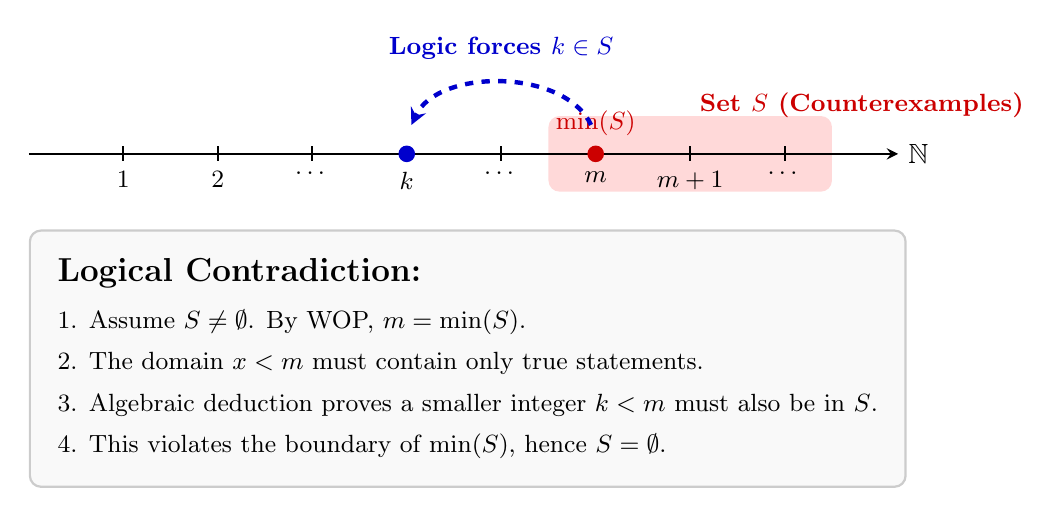
\begin{tikzpicture}[scale=1.2, >=stealth]

    % 1. LAYER 1: Background Set Shading
    \fill[red!15, rounded corners=4pt] (5.5, -0.4) rectangle (8.5, 0.4);

    % 2. LAYER 2: Crisp Number Line Axis 
    \draw[thick, ->] (0,0) -- (9.2,0) node[right, black] {$\mathbb{N}$};
    
    % 3. LAYER 3: Axis Ticks & Clean Decoupled Labels
    \foreach \x in {1,2,3,4,5,6,7,8} {
        \draw[thick] (\x, 0.08) -- (\x, -0.08);
    }
    \node[below=3pt, font=\small] at (1,0) {$1$};
    \node[below=3pt, font=\small] at (2,0) {$2$};
    \node[below=3pt, font=\small] at (3,0) {$\dots$};
    \node[below=3pt, font=\small] at (4,0) {$k$};
    \node[below=3pt, font=\small] at (5,0) {$\dots$};
    \node[below=3pt, font=\small] at (6,0) {$m$};
    \node[below=3pt, font=\small] at (7,0) {$m+1$};
    \node[below=3pt, font=\small] at (8,0) {$\dots$};

    % Point vectors sitting on the line
    \fill[blue!80!black] (4,0) circle (2.5pt);
    \fill[red!80!black] (6,0) circle (2.5pt);

    % 4. LAYER 4: Clear Upper Labels
    % Locked directly over the red minimum element
    \node[above=3pt, red!80!black, font=\small] at (6,0) {$\min(S)$};

    % THE ULTIMATE FIX: Anchor=west locks the left edge at x=7.0, forcing rightward growth completely away from the arrow
    \node[red!80!black, above=4pt, font=\small, anchor=west] at (7.0, 0.4) {\textbf{Set $S$ (Counterexamples)}};

    % 5. LAYER 5: The Deduction Arc & High-Altitude Label
    \draw[->, ultra thick, blue!80!black, dashed, shorten <=4pt, shorten >=4pt] 
        (6, 0.2) to[out=115, in=65] (4, 0.2);
        
    \node[blue!80!black, above, font=\small\bfseries] at (5.0, 0.9) {Logic forces $k \in S$};

    % 6. LAYER 6: Master Dynamic Contradiction Box
    \node[
        draw=gray!40,
        thick,
        fill=gray!5,
        rounded corners=4pt,
        inner sep=10pt,
        align=left,
        anchor=north west,  
        font=\small
    ] at (0, -0.8) {      
        \textbf{\large Logical Contradiction:} \\[6pt]
        1. Assume $S \neq \emptyset$. By WOP, $m = \min(S)$. \\[4pt]
        2. The domain $x < m$ must contain only true statements. \\[4pt]
        3. Algebraic deduction proves a smaller integer $k < m$ must also be in $S$. \\[4pt]
        4. This violates the boundary of $\min(S)$, hence $S = \emptyset$.
    };
\end{tikzpicture}
\end{center}


\subsection{Heuristics \& "Cheats"}
\begin{itemize}
    \item \textbf{When to use Minimum Counterexample?} If a problem involves proving the \textit{existence} of a decomposition (like binary representation or prime factorization), Minimum Counterexample is vastly superior to standard induction because you don't need to build $m$ from $m-1$; you can break $m$ down into \textit{any} smaller components and rely on their minimality.
    \item \textbf{The $\Delta$ Shortcut:} For divisibility proofs $d \mid f(n)$, immediately compute $f(m) - f(m-1)$. If you can prove $d$ divides this difference, the proof is essentially complete.
\end{itemize}

\subsection{Pitfalls \& Fallacies}
\begin{itemize}
    \item \textbf{The Base Case Boundary Violation:} The most common fatal flaw is assuming $m-1$ is a valid positive integer without first proving that $m$ cannot be the base case (e.g., $m=1$). If $m=1$, then $m-1=0$, which may lie outside the domain of $\N$, rendering the inductive step logically void.
    \item \textbf{Affirming the Consequent:} Assuming $P(m)$ is true to prove $P(m-1)$ is true. You must assume $P(m)$ is \textit{false} and use the \textit{truth} of $P(m-1)$ to find a contradiction.
\end{itemize}

\newpage
\section{Conceptual Synthesis and The "Big Picture"}

\subsection{A) Thematic Connections}
The central theme of this topic is the \textbf{topological rigidity of discrete spaces}. In continuous spaces like $\R$, there is no "next" or "previous" element, meaning the Well-Ordering Principle fails entirely (e.g., the open interval $(0,1)$ has no minimum). By establishing that $\N$ is well-ordered, we bridge basic arithmetic to advanced set theory. The Minimum Counterexample method is practically an isomorphism to the Axiom of Choice for countable sets, allowing us to "select" a definitive starting point for any property that fails.

\subsection{B) Forward and Backward Links}
\begin{itemize}
    \item \textbf{Backward Links:} This topic rigorously formalizes the intuitive "domino effect" taught in introductory logic. It replaces the mechanical $k \to k+1$ engine of standard induction with a pure set-theoretic argument.
    \item \textbf{Forward Links:} Understanding well-ordered sets is the absolute bedrock for \textbf{Transfinite Induction} in set theory (dealing with ordinal numbers beyond infinity, $\omega, \omega+1, \dots$). Furthermore, in Measure Theory and Probability, the concept of a "first time" an event occurs (a Stopping Time) relies entirely on the well-ordering of discrete time steps.
\end{itemize}

\section{Abstract Real-World Modeling (AI, ML, \& Quant Finance)}

\subsection{A) Concrete Scenarios}
\begin{enumerate}
    \item \textbf{Quantitative Finance (Default Risk \& Stopping Times):} In stochastic calculus, modeling the exact moment a firm goes bankrupt is modeled as a "First Hitting Time." Because discrete trading days form a well-ordered set, we are mathematically guaranteed that if a firm defaults within a year, there is a strict, identifiable \textit{minimum} day $m$ on which the asset price crossed the default threshold.
    \item \textbf{Artificial Intelligence (Halting Problem \& Loop Invariants):} In algorithmic verification, proving that an AI planning algorithm will eventually terminate (halt) relies on constructing a "variant" function that maps the state space to $\N$. Because $\N$ is well-ordered, the sequence of states must eventually reach a minimum (termination), preventing infinite loops.
\end{enumerate}

\subsection{B) Model Problem Setup: Stochastic Stopping Times}
Let us formalize the Quantitative Finance scenario. Let $(\Omega, \F, \Prob)$ be a probability space equipped with a discrete-time filtration $\F = (\F_n)_{n \in \N}$. Let $X = (X_n)_{n \in \N}$ be an adapted stochastic process representing the daily log-return of a derivative asset. 

Define a critical barrier $B \in \R$ (the default threshold). We define the random variable $\tau : \Omega \to \N \cup \{\infty\}$ as the \textbf{first hitting time} of the barrier:
\[
\tau(\omega) = \min \{ n \in \N : X_n(\omega) \le B \}
\]
\textbf{Theoretical Framework:} How do we know $\tau$ is a well-defined random variable? 
For any sample path $\omega \in \Omega$, let $S(\omega) = \{ n \in \N : X_n(\omega) \le B \}$. 
If the asset never defaults, $S(\omega) = \emptyset$, and we define $\tau(\omega) = \infty$. 
If the asset \textit{does} default, then $S(\omega) \neq \emptyset$. Because $S(\omega) \subseteq \N$, the \textbf{Well-Ordering Principle} guarantees that $S(\omega)$ has a unique minimum element. Thus, the $\min$ operator is rigorously justified, and $\tau(\omega)$ exists and is unique. 

Furthermore, to prove that $\tau$ is a valid stopping time, we must show that the event $\{\tau = n\} \in \F_n$. 
Using the logic of the minimum counterexample, if $n$ is the minimum, then for all $k < n$, the event did not occur. Thus:
\[
\{\tau = n\} = \{X_n \le B\} \cap \left( \bigcap_{k=1}^{n-1} \{X_k > B\} \right)
\]
Since $X$ is adapted, each $\{X_k > B\} \in \F_k \subseteq \F_n$. Thus, the intersection belongs to $\F_n$, proving $\tau$ is a stopping time, allowing the application of the Optional Stopping Theorem for martingale pricing.

\newpage
\section{Common Variations and Untested Concepts}

A critical variation of the Minimum Counterexample not explicitly tested in the homework is \textbf{Fermat's Method of Infinite Descent}. While Minimum Counterexample assumes a smallest element and finds a contradiction by going one step backward to $m-1$, Infinite Descent assumes a solution exists and algebraically constructs a strictly smaller solution, creating an infinite decreasing sequence in $\N$, which violates the WOP.

\textbf{Missing Concept Example: Proving Irrationality}
\begin{theorem}
$\sqrt{2}$ is irrational.
\end{theorem}
\begin{proof}
Assume, to the contrary, that $\sqrt{2}$ is rational. Then there exists a set of positive integers $S = \{ a \in \N : \exists b \in \N, \sqrt{2} = \frac{a}{b} \}$.
Since $S$ is non-empty, by the Well-Ordering Principle, it has a minimum element, say $a$. Let the corresponding denominator be $b$.
Squaring both sides yields $2 = \frac{a^2}{b^2}$, so $a^2 = 2b^2$.
This implies $a^2$ is even, which necessitates that $a$ is even. Let $a = 2k$ for some $k \in \N$.
Substitute this back: $(2k)^2 = 2b^2 \implies 4k^2 = 2b^2 \implies b^2 = 2k^2$.
This implies $b^2$ is even, so $b$ is even. Let $b = 2j$ for some $j \in \N$.
We now have $\sqrt{2} = \frac{a}{b} = \frac{2k}{2j} = \frac{k}{j}$.
Thus, $k \in S$. However, $k = \frac{a}{2} < a$. This contradicts the assumption that $a$ was the minimum element of $S$. Therefore, $S = \emptyset$, and $\sqrt{2}$ is irrational.
\end{proof}

\section{Advanced Diagnostic Testing: "Find the Flaw"}

Below are five proofs using the Minimum Counterexample method that contain a subtle, critical logical flaw. Act as the grader: identify the error and explain the resolution.

\subsection{Flawed Proofs}
\begin{enumerate}
    \item \textbf{Claim:} For all $n \in \N$, $n = n+1$.
    \textit{Proof:} Assume false. Let $m$ be the smallest counterexample. Since $m$ is minimal, the statement holds for $m-1$. Thus, $m-1 = (m-1) + 1 \implies m-1 = m$. Adding $1$ to both sides gives $m = m+1$. This means the statement holds for $m$, contradicting that $m$ is a counterexample. $\blacksquare$
    
    \item \textbf{Claim:} For all $n \in \N$, $3^n > n^3$.
    \textit{Proof:} Assume false. Let $m$ be the smallest counterexample. For $n=1$, $3^1 > 1^3$ (True). For $n=2$, $3^2 > 2^3 \implies 9 > 8$ (True). Thus $m \ge 3$. By minimality, $3^{m-1} > (m-1)^3$. Multiplying by 3 gives $3^m > 3(m-1)^3 = 3m^3 - 9m^2 + 9m - 3$. For $m \ge 3$, $3m^3 - 9m^2 + 9m - 3 > m^3$. Thus $3^m > m^3$, contradiction. $\blacksquare$
    
    \item \textbf{Claim:} For all $n \in \N$, $4 \mid (n^2 + 3)$.
    \textit{Proof:} Assume false. Let $m$ be the smallest counterexample. For $n=1$, $1^2+3=4$, $4 \mid 4$ (True). So $m \ge 2$. By minimality, $4 \mid ((m-2)^2 + 3)$. Expanding: $(m-2)^2 + 3 = m^2 - 4m + 4 + 3 = (m^2 + 3) - 4(m - 1)$. Since $4$ divides the left side and $4$ divides $4(m-1)$, $4$ must divide $m^2 + 3$. Contradiction. $\blacksquare$
    
    \item \textbf{Claim:} Every positive integer $n$ can be written as $2x + 3y$ for non-negative integers $x, y$.
    \textit{Proof:} Assume false. Let $m$ be the smallest counterexample. For $n=1$, it fails. Wait, let's check $n=2$: $2(1)+3(0)=2$. $n=3$: $2(0)+3(1)=3$. Let $m$ be the smallest counterexample $m \ge 4$. By minimality, $m-2$ can be written as $2x+3y$. Then $m = (m-2)+2 = 2x+3y+2 = 2(x+1)+3y$. Thus $m$ can be written this way. Contradiction. $\blacksquare$
    
    \item \textbf{Claim:} All horses are the same color.
    \textit{Proof:} Let $S$ be the set of integers $n$ where a set of $n$ horses has multiple colors. Let $m$ be the minimum of $S$. $m \neq 1$ trivially. So $m \ge 2$. Take a set of $m$ horses. Remove one; the remaining $m-1$ are the same color by minimality. Swap the removed horse with another; those $m-1$ are the same color. Thus all $m$ are the same color. Contradiction. $\blacksquare$
\end{enumerate}

\subsection{Solution Key (Grader's Resolution)}
\begin{enumerate}
    \item \textbf{Flaw:} The base case was never checked. If $m=1$ is the minimum counterexample, then $m-1 = 0$, which is not in $\N$. The inductive hypothesis cannot be applied to $0$.
    \item \textbf{Flaw:} The bounding algebra fails at $m=3$. The proof claims $3m^3 - 9m^2 + 9m - 3 > m^3 \implies 2m^3 - 9m^2 + 9m - 3 > 0$. If $m=3$, $2(27) - 9(9) + 9(3) - 3 = 54 - 81 + 27 - 3 = -3 \ngtr 0$. The claim is actually false ($3^3 = 27$, $3^3 = 27$, not strictly greater).
    \item \textbf{Flaw:} The proof assumes the statement holds for $m-2$. However, if $m=2$ is the minimum counterexample, $m-2 = 0$, which is outside the domain $\N$. The claim is false for $n=2$ ($2^2+3=7$, not divisible by 4).
    \item \textbf{Flaw:} The proof correctly identifies that $n=1$ fails, but then arbitrarily redefines the minimum counterexample to be $m \ge 4$ without proving the statement for $n=1$. The claim is simply false for $n=1$.
    \item \textbf{Flaw:} The overlapping sets argument fails when $m=2$. If you have 2 horses, removing one leaves a set of 1 (color A). Swapping leaves a different set of 1 (color B). There is no intersection between these two sets of size 1 to force color A = color B.
\end{enumerate}

\end{document}